\begin{tikzpicture}[scale=1.5]

    \node at (-2,1) {$\sfrac{\mathscr{U}}{\sim}$};

    \draw[thick] (0,0) node{...} ellipse (2 and 1);
    \draw (-1.25,-.78) -- (-1.25,.78);
    \draw (-.5,-.97) -- (-.5,.97);
    \draw (.5,-.97) -- (.5,.97);
    \draw (1.25,-.78) -- (1.25,.78);

    \draw[fill,blue] (-.875,0) circle (.02);
    \draw[->,blue] (-.875,0) -- (-1.75,-1);
    \node[blue,below] at (-1.75,-1) {Classe di equivalenza};

\end{tikzpicture}